\documentclass{beamer}
\usepackage{graphicx}
\usepackage{epstopdf}

% \usetheme{Rochester}
% \usecolortheme{orchid}
% % \usefonttheme{structuresmallcapsserif}
% \usefonttheme{focus}

\title{$P$-Wave Charmonia Production in Exclusive $B_c$-Meson Decays}
\author{Alexey Luchinsky}
\institute{IHEP, Russia\\ BGSU, Bowling Green, OH, USA}


\newcommand{\R}{\mathcal{R}}
\newcommand{\M}{\mathcal{M}}
\newcommand{\A}{\mathcal{A}}
	
\newcommand{\cc}{(\bar{c}c)}
	
\graphicspath{{figs/}}

\begin{document}

\begin{frame}
  \maketitle
\end{frame}

\section{Introduction}
\begin{frame}
  \frametitle{Introduction}
  \begin{itemize}
  \item $B_c^+ = (\bar{b}c)$ combines both charmonia and bottomonia properties
  \item Can be used to
    \begin{itemize}
    \item study QCD in confinment and assymtotoc freedom regimes
    \item check existing models for heavy quarkonia description      
    \end{itemize}
  \item $B_c \to \cc+\R$ decays can be studied using the factorization model
  \item Good results for vector charmonia:
    \begin{itemize}
    \item $B_c \to \psi^{(')} + e\nu, \pi, \rho, 3\pi, \dots$
    \end{itemize}
  \item What about $P$-wave states
    \begin{itemize}
    \item $B_c \to \chi_{cJ} + e\nu, \pi, \rho, 3\pi, \dots$
    \end{itemize}

  \end{itemize}
\end{frame}


\begin{frame}
  \frametitle{Content}
  \tableofcontents
\end{frame}



\section{$B_c\to \cc + \R$}

\begin{frame}[t]
  \frametitle{Factorization}
  Diagram and amplitude factorise:
  \begin{center}
    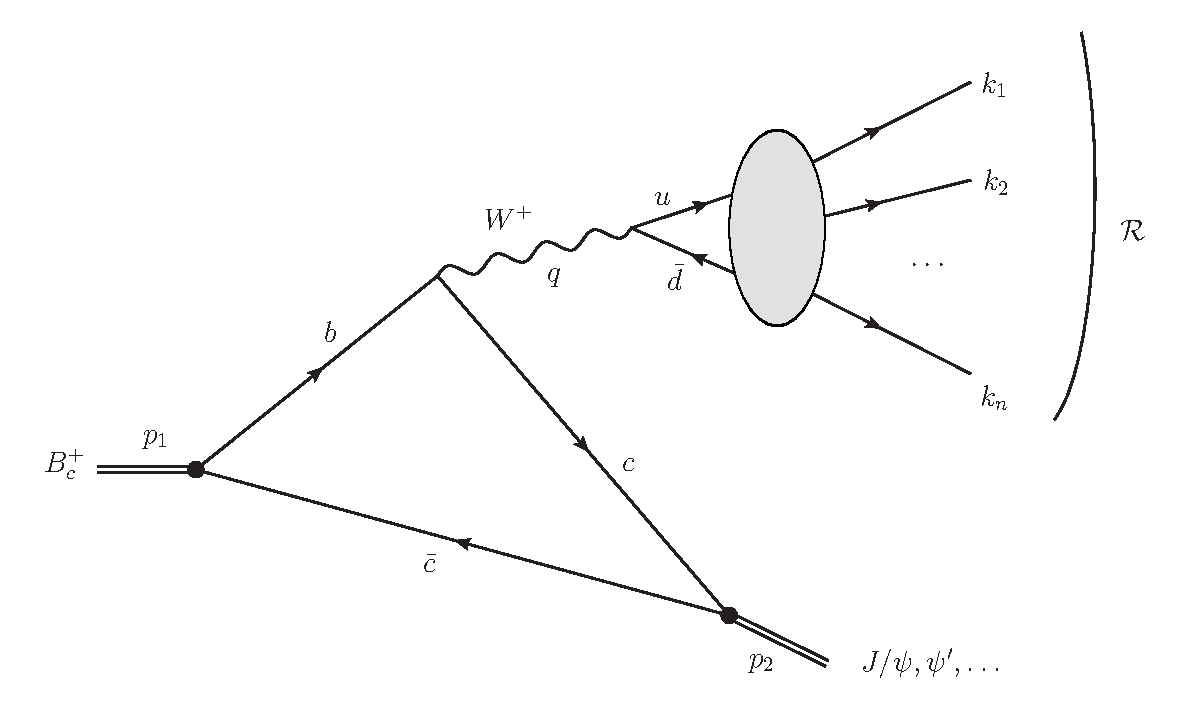
\includegraphics[width=0.5\columnwidth]{diags_BcCCW}
  \end{center}
      $$\M\left(B_c \to J/\psi + \R\right) = H^\mu \epsilon^{(\R)}_\mu$$
   where
   \begin{itemize}
   \item $H^\mu$ is the $B_c\to J/\psi W$ transition vertex
   \item $\epsilon^{(\R)}_\mu$ is effective  $W\to\R$ polarization vector
   \end{itemize}
The differential width is
$$
\frac{d\Gamma}{dq^2} \sim \frac{d\Gamma_T}{dq^2} \rho_T\left(q^2\right) + \frac{d\Gamma_L}{dq^2} \rho_L\left(q^2\right)
$$
\end{frame}


\begin{frame}
  \frametitle{$B_c \to J/\psi W$ transition}
  Lots of articles, e.g. [Ebert, Faustov, Galkin,     Phys.Rev.D 68 (2003) 094020]
  \begin{align*}
    \label{eq:1}
    H_\mu =& \frac{2i V(q^2)}{M_1+M_2}e_{\mu\nu\rho\sigma}\epsilon^\nu p_1^\rho p_2^\sigma
             + (M_1+M_2) A_1(q^2)\epsilon_\mu - \\
     & A_2(q^2) \left[p_{1\mu} + p_{2\mu}-\frac{M_1^2-M_2^2}{q^2}q^\mu\right]\frac{\epsilon q}{M_1+M_2}
  \end{align*}
  \centering{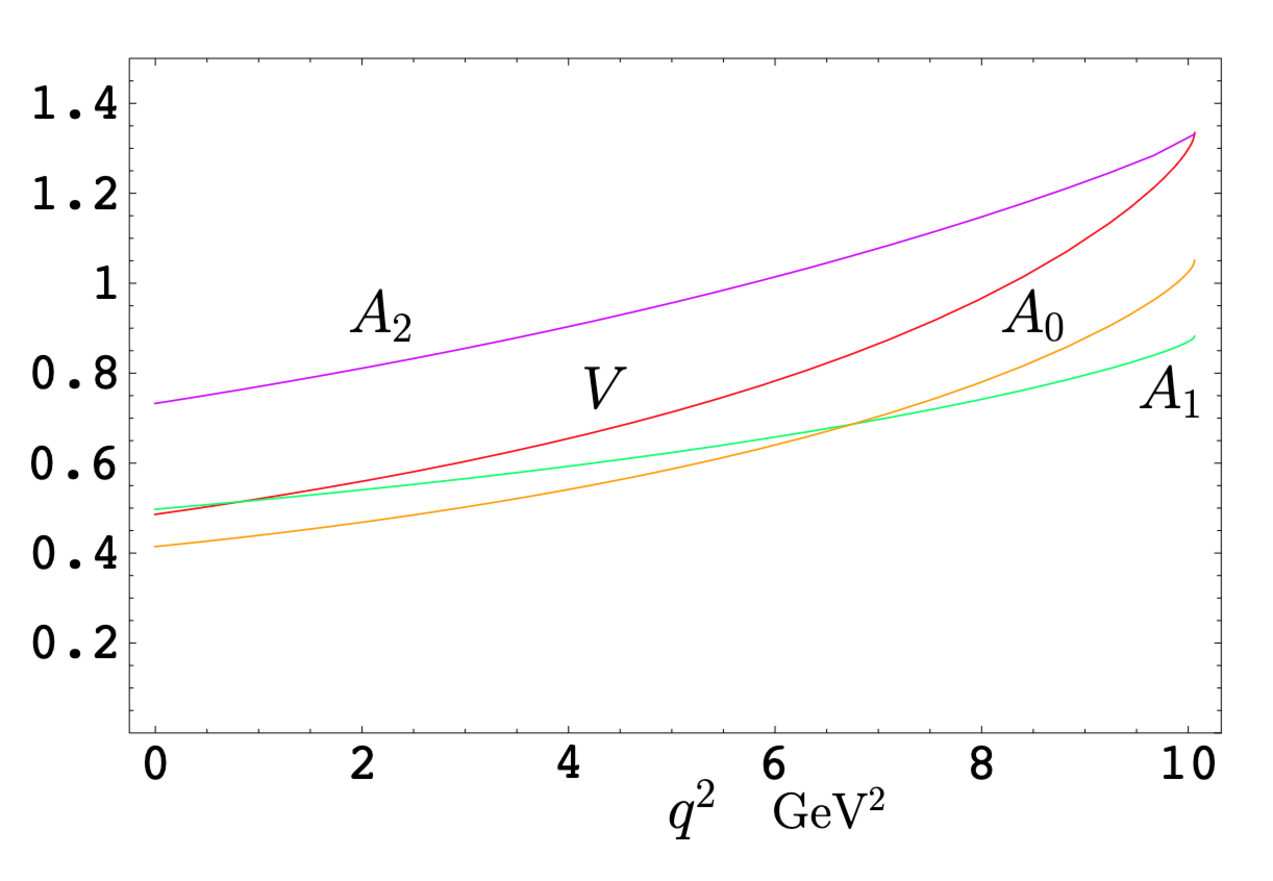
\includegraphics[width=0.7\textwidth]{0306306_Fig6}}
\end{frame}


\begin{frame}
  \frametitle{$W \to  2\pi$}
  \begin{columns}
    \begin{column}{0.5\textwidth}
      % diag grabbed from arXiv:1104.0808
      \centering{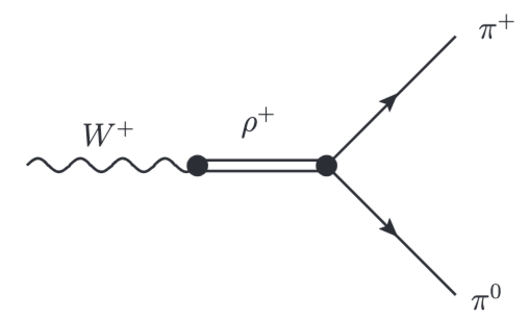
\includegraphics[width=0.9\textwidth]{diag_W_2pi}}
    \end{column}
    \begin{column}{0.5\textwidth}
  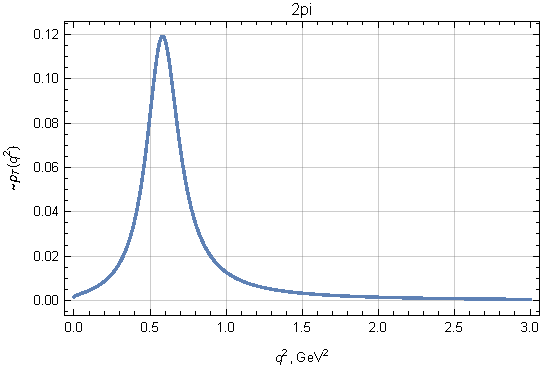
\includegraphics[width=0.9\textwidth]{figs/rhoT_2pi_q2}
    \end{column}
  \end{columns}
\end{frame}


\begin{frame}
  \frametitle{$W \to   3\pi$}
  \begin{columns}
    \begin{column}{0.5\textwidth}
      % diag grabbed from arXiv:1104.0808
      \centering{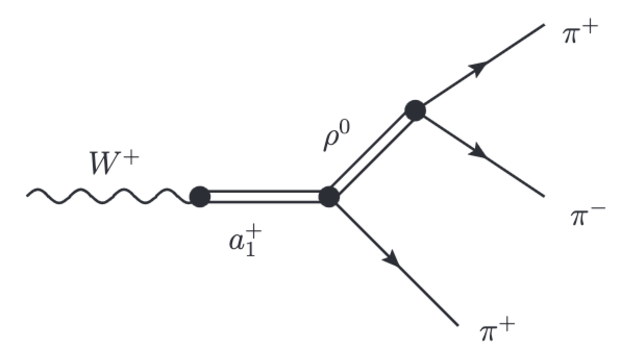
\includegraphics[width=0.9\textwidth]{diag_W_3pi}}
    \end{column}
    \begin{column}{0.5\textwidth}
      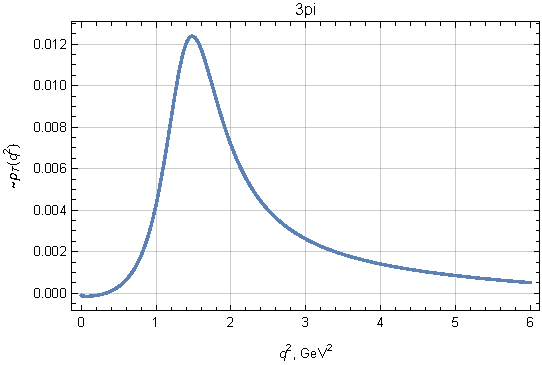
\includegraphics[width=0.9\textwidth]{figs/rhoT_3pi_q2}

      {\tiny Agrees with CERN arXiv 1204.0079 [hep-ex]}
      
      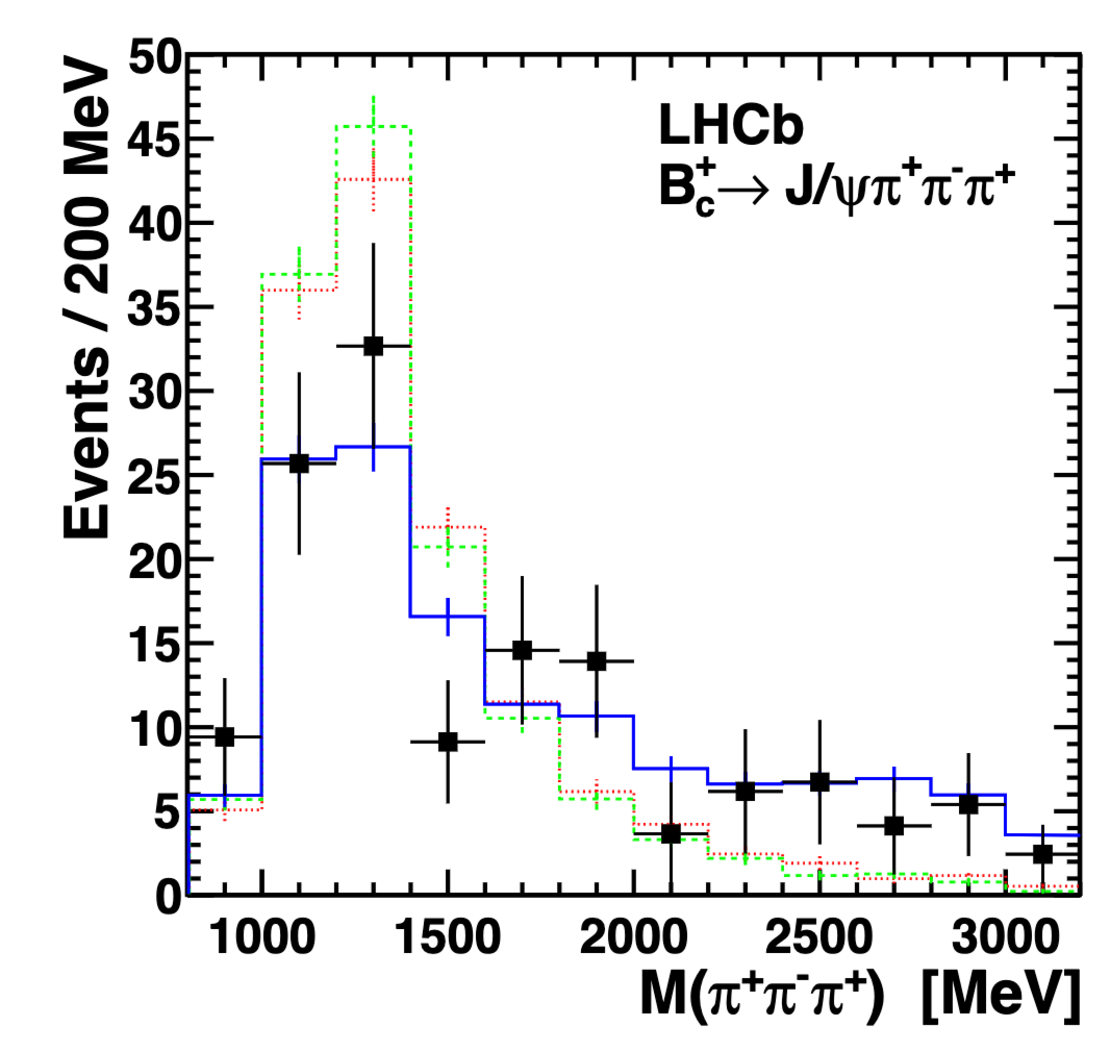
\includegraphics[width = 0.9\textwidth]{1204_0079_Fig2}
    \end{column}
  \end{columns}
\end{frame}

\begin{frame}
  \frametitle{$W \to   5\pi$}
    \begin{columns}
    \begin{column}{0.5\textwidth}
      % diag grabbed from arXiv:1208.1398
      \centering{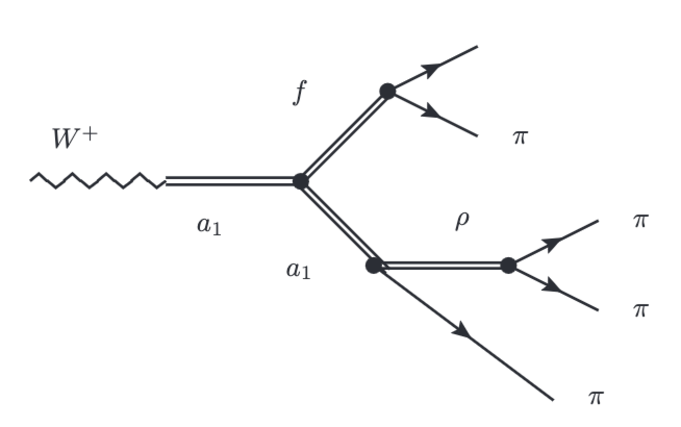
\includegraphics[width=0.9\textwidth]{diag_W_5pi}}
    \end{column}
    \begin{column}{0.5\textwidth}
      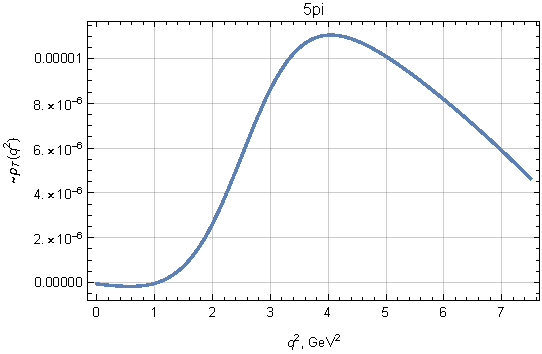
\includegraphics[width=0.9\textwidth]{figs/rhoT_5pi_q2}
      {\tiny Agrees with CERN [2208.08660 [hep-ex]]}
      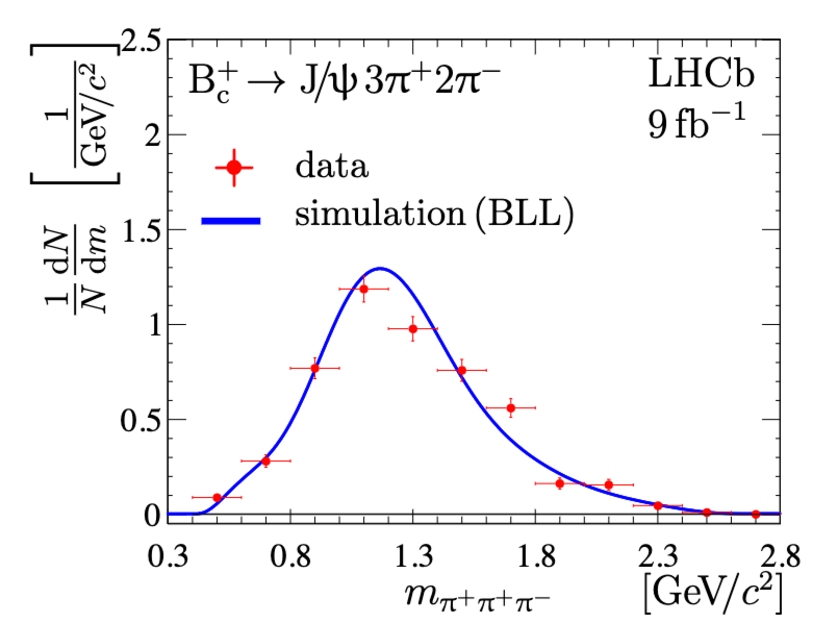
\includegraphics[width=0.9\textwidth]{figs/2208_08660_Fig4}      
    \end{column}
  \end{columns}

\end{frame}


\section{$B_c\to \chi_{cJ}+\R$}
\begin{frame}
  \frametitle{$B_c\to \chi_{cJ}+\R$}
\begin{center}
  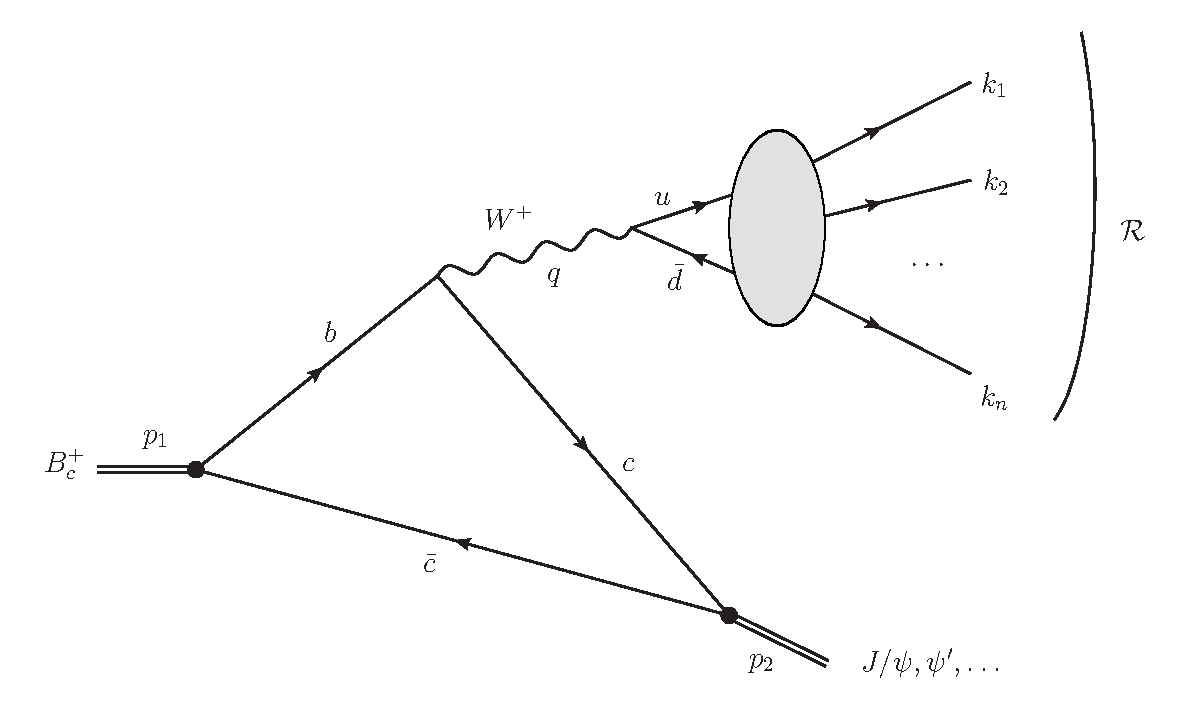
\includegraphics[width=0.5\columnwidth]{diags_BcCCW}
\end{center}
$$\M\left(B_c \to \chi_{cJ} + \R\right) = H^\mu \epsilon^{(\R)}_\mu$$
Form-factors of the $B_c\to \chi_{cJ}W$ transitions were considered in
\begin{itemize}
\item D. Ebert, R. N. Faustov, V. O. Galkin, PRD 82 (2010) 034019 
\item Zhi-hui Wang et al,  	J. Phys. G,  39 (2012) 015009
\item E. Hernandez et al, PRD      74 (2006) 074008
\item etc.
\end{itemize}
I will use these form factors, compare published branching fractions and consider some other decay modes
\end{frame}

\subsection{$\chi_{c0}$}
\begin{frame}
  \frametitle{$\chi_{c0}$, Form Factors}
  $$
  H_\mu = f_{+}\left(q^2\right) \left(p_1+p_2\right)_\mu + f_{-}\left(q^2\right) \left(p_1-p_2\right)_\mu 
  $$
  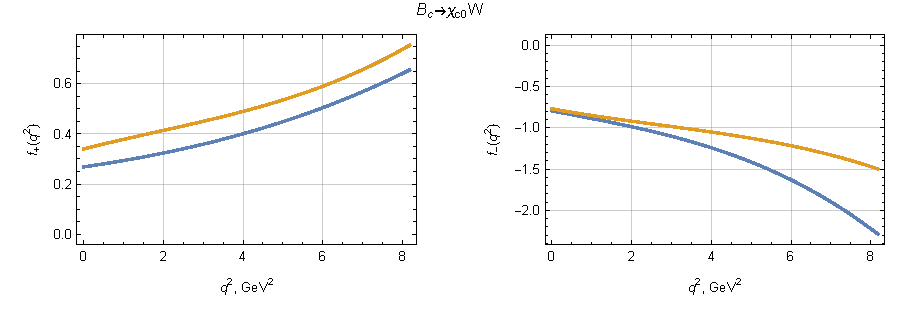
\includegraphics[width=0.9\textwidth]{figs/ff_chi_c0}

  $f_{-}(q^2)$ gives no contribution to most of the decays
  
  $f_{+}(q^2)$ are proportional to each other
\end{frame}

\newcommand{\Br}{\mathrm{Br}}

\begin{frame}
  \frametitle{$B_c \to \chi_{c0} \pi$}
  \begin{columns}
    \begin{column}{0.5\textwidth}
      \centering{[Ebert]:}
      % Bc -> chi_c0 + P with [Ebert]
      \begin{tabular}{lcr}
          Paper &:& $\Br  = 0.021\%$ \\
          this      &:& $\Br  = 0.022\%$ \\
		  ratio   &:& $1.034$ \\
      \end{tabular}

    \end{column}
    \begin{column}{0.5\textwidth}
      \centering{[Wang]:}
      % Bc -> chi_c0 + P with [Wang]
      \begin{tabular}{lcr}
          Paper &:& $\Br  = 0.031\pm 0.004\%$ \\
          this      &:& $\Br  = 0.035\%$ \\
		  ratio   &:& $1.127\pm 0.145$ \\
      \end{tabular}

    \end{column}
  \end{columns}
  \vspace{2cm}
  Good agreement
\end{frame}

\newcommand{\VSpace}{}

\begin{frame}[t]
  \frametitle{$B_c \to \chi_{c0} e \nu$}
  \begin{columns}
    \begin{column}{0.5\textwidth}
      \centering{[Ebert]}
      % Bc -> chi_c0 + enu with [Ebert]
      \begin{tabular}{lcr}
          Paper &:& $\Br  = 0.087\%$ \\
          this      &:& $\Br  = 0.087\%$ \\        
      \end{tabular}

      \VSpace 
      \visible<2->{      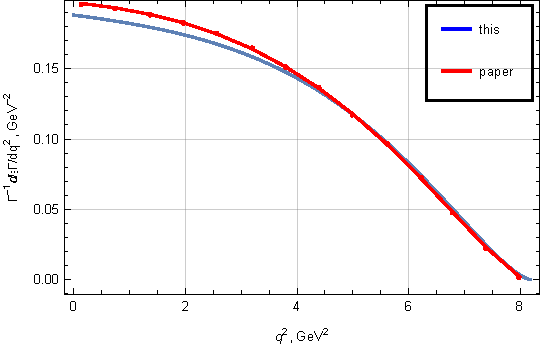
\includegraphics[width=0.9\textwidth, height = 0.55\textheight]{chi_c0_enu_q2_Ebert}}
    \end{column}
    \begin{column}{0.5\textwidth}
      \only<3->{
        \centering{[Wang]}
        % Bc -> chi_c0 + enu with [Wang]
      \begin{tabular}{lcr}
          Paper &:& $\Br  = 0.13\pm 0.03\%$ \\
          this      &:& $\Br  = 0.179\%$ \\
		  ratio   &:& $1.375\pm 0.317$ \\
      \end{tabular}

      }
      \VSpace 
      \only<3,4>{\visible<4>{      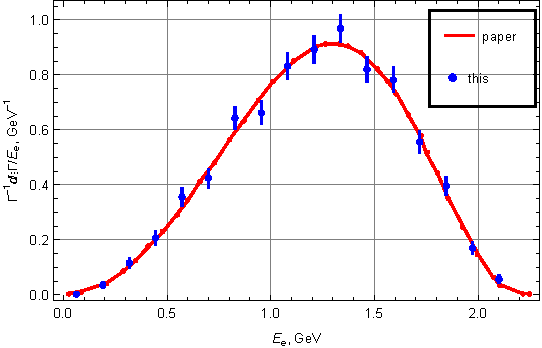
\includegraphics[width=0.9\textwidth, height = 0.55\textheight]{chi_c0_enu_e2_Wang}}}
      \only<5>{      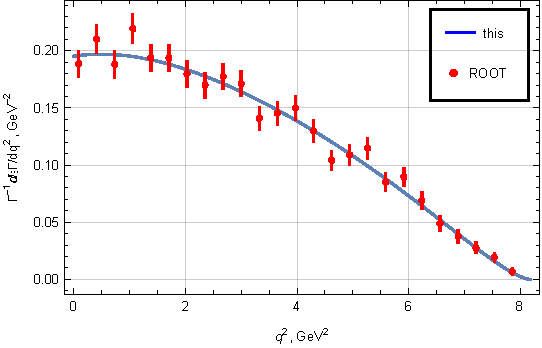
\includegraphics[width=0.9\textwidth, height = 0.55\textheight]{chi_c0_enu_q2_Wang}}
    \end{column}
  \end{columns}
\end{frame}

\begin{frame}
  \frametitle{$B_c \to \chi_{c0} \rho$}
  $$
  \Br\left[B_c \to \chi_{c0} \rho\right] =
  6\pi^2 f_\rho^2 \left.
    \frac{d\Br\left(B_c\to\chi_{c0}+e\nu\right)}{dq^2}
  \right|_{q^2=m_\rho^2}
  $$
  \begin{columns}
    \begin{column}{0.5\textwidth}
      \centering{Ebert}
      \vspace{3mm}
      \centering{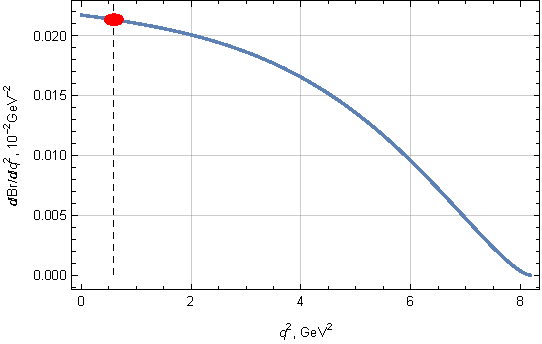
\includegraphics[width=0.9\textwidth]{chi_c0_enu_rho_Ebert}}
      % Bc -> chi_c0 + V with [Ebert]
      \begin{tabular}{lcr}
          Paper &:& $\Br  = 0.058\%$ \\
          this      &:& $\Br  = 0.042\%$ \\
		  ratio   &:& $0.726$ \\
      \end{tabular}

    \end{column}
  \begin{column}{0.5\textwidth}
      \centering{Wang}\\
      \vspace{3mm}
      \centering{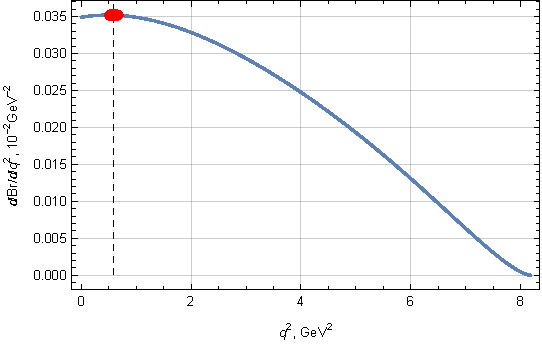
\includegraphics[width=0.9\textwidth]{chi_c0_enu_rho_Wang}}
      % Bc -> chi_c0 + V with [Wang]
      % Bc -> chi_c0 + V with [Wang]
      \begin{tabular}{lcr}
          Paper &:& $\Br  = 0.076\pm 0.009\%$ \\
          this      &:& $\Br  = 0.09\%$ \\
		  ratio   &:& $1.186\pm 0.14$ \\
      \end{tabular}

       \end{column}
\end{columns}
\end{frame}

\subsection{$\chi_{c1}$}
\begin{frame}
  \frametitle{$\chi_{c1}$, Form Factors}
  \begin{align*}
    H_\mu =& \frac{2i h_A(q^2)}{M_1+M_2}e_{\mu\nu\rho\sigma}\epsilon^\nu p_1^\rho p_2^\sigma
             + (M_1+M_2) h_{V_1}(q^2)\epsilon_\mu + \\
     & [h_{V_2}(q^2)p_{1\mu} + h_{V_3}(q^2)p_{2\mu}]\frac{\epsilon q}{M_1}
  \end{align*}
  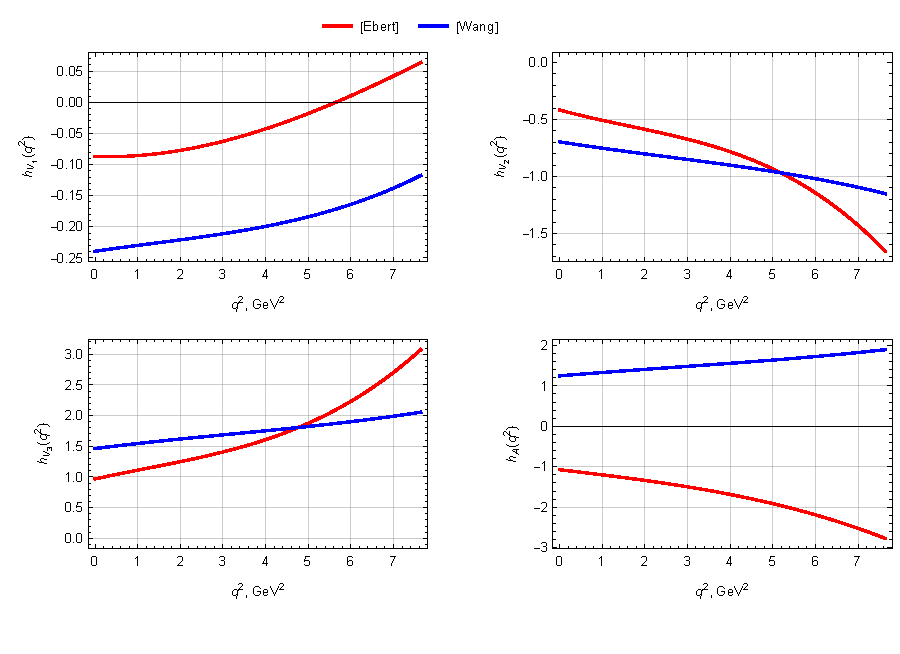
\includegraphics[width=0.8\textwidth]{figs/ff_chi_c1}
\end{frame}

\begin{frame}
  \frametitle{$B_c \to \chi_{c1} \pi$}
  \begin{columns}
    \begin{column}{0.5\textwidth}
      \centering{[Ebert]:}
      % Bc -> chi_c1 + P with [Ebert]
      \begin{tabular}{lcr}
          Paper &:& $\Br  = 0.02\%$ \\
          this      &:& $\Br  = 0.001\%$ \\
		  ratio   &:& $0.031$ \\
      \end{tabular}

    \end{column}
    \begin{column}{0.5\textwidth}
      \centering{[Wang]:}
      % Bc -> chi_c1 + P with [Wang]
      \begin{tabular}{lcr}
          Paper &:& $\Br  = 0.002\pm 0.\%$ \\
          this      &:& $\Br  = 0.002\pm 0.001\%$ \\        
      \end{tabular}

    \end{column}
  \end{columns}
\end{frame}


\begin{frame}[t]
  \frametitle{$B_c \to \chi_{c1} e \nu$}
  \begin{columns}
    \begin{column}{0.5\textwidth}
      \centering{[Ebert]}
      % Bc -> chi_c1 + enu with [Ebert]
      \begin{tabular}{lcr}
          Paper &:& $\Br  = 0.082\%$ \\
          this      &:& $\Br  = 0.082\%$ \\        
      \end{tabular}

      \VSpace 
      \visible<2->{      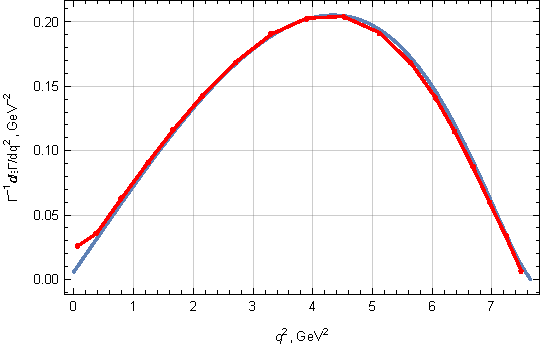
\includegraphics[width=0.9\textwidth, height = 0.55\textheight]{chi_c1_enu_q2_Ebert}}
    \end{column}
    \begin{column}{0.5\textwidth}
      \only<3->{
        \centering{[Wang]}
      % Bc -> chi_c1 + enu with [Wang]
      \begin{tabular}{lcr}
          Paper &:& $\Br  = 0.11\pm 0.03\%$ \\
          this      &:& $\Br  = 0.149\%$ \\
		  ratio   &:& $1.355\pm 0.369$ \\
      \end{tabular}

      }
      \VSpace 
      \only<3,4>{\visible<4>{      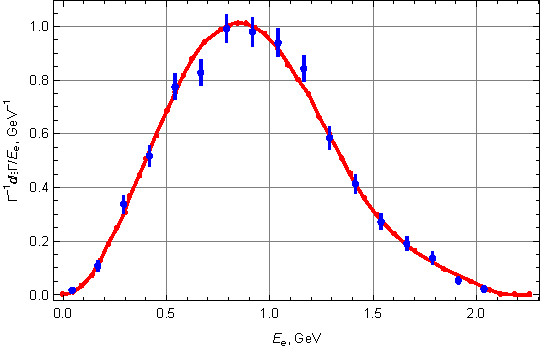
\includegraphics[width=0.9\textwidth, height = 0.55\textheight]{chi_c1_enu_e2_Wang}}}
      \only<5>{      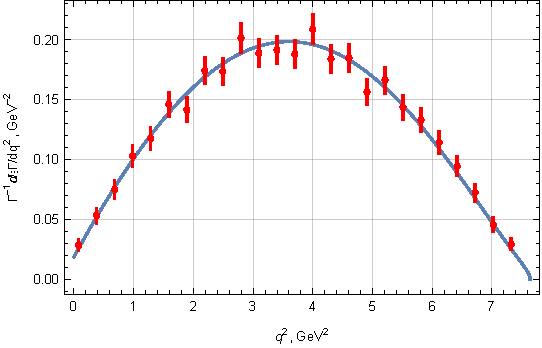
\includegraphics[width=0.9\textwidth, height = 0.55\textheight]{chi_c1_enu_q2_Wang}}
    \end{column}
  \end{columns}
\end{frame}


\begin{frame}
  \frametitle{$B_c \to \chi_{c1} \rho$}
  $$
  \Br\left[B_c \to \chi_{c1} \rho\right] =
  6\pi^2 f_\rho^2 \left.
    \frac{d\Br\left(B_c\to\chi_{c1}+e\nu\right)}{dq^2}
  \right|_{q^2=m_\rho^2}
  $$
  \begin{columns}
    \begin{column}{0.5\textwidth}
      \centering{Ebert}
      \vspace{3mm}
      \centering{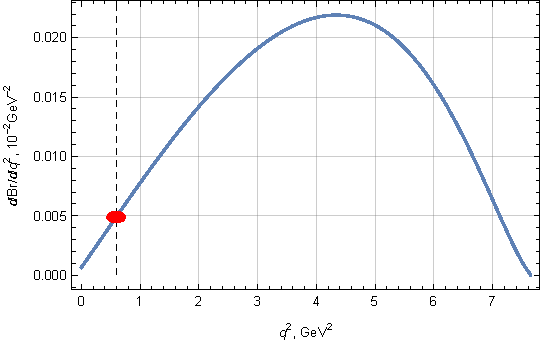
\includegraphics[width=0.9\textwidth]{chi_c1_enu_rho_Ebert}}
      % Bc -> chi_c1 + V with [Ebert]
      \begin{tabular}{lcr}
          Paper &:& $\Br  = 0.015\%$ \\
          this      &:& $\Br  = 0.009\%$ \\        
      \end{tabular}

    \end{column}
  \begin{column}{0.5\textwidth}
      \centering{Wang}\\
      \vspace{3mm}
      \centering{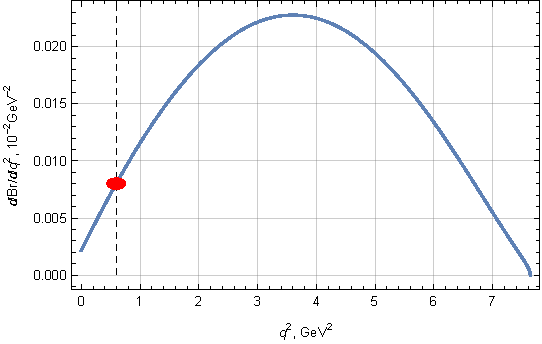
\includegraphics[width=0.9\textwidth]{chi_c1_enu_rho_Wang}}
      % Bc -> chi_c1 + V with [Wang]
      \begin{tabular}{lcr}
          Paper &:& $\Br  = 0.023\pm 0.002\%$ \\
          this      &:& $\Br  = 0.018\pm 0.005\%$ \\        
      \end{tabular}

    \end{column}
\end{columns}
\end{frame}


\subsection{$\chi_{c2}$}
\begin{frame}
  \frametitle{$\chi_{c2}$, Form Factors}
  \begin{align*}
  H_\mu &=
\frac{2it_V(q^2)}{M_1+M_2} \epsilon^{\mu\nu\rho\sigma}\epsilon^*_{\nu\alpha}
          \frac{p_1^\alpha}{M_1}  p_1 p_1  
     +  (M_1+M_2)t_{A_1}(q^2)\epsilon^{*\mu\alpha}\frac{p_{1\alpha}}{M_1} +\\
&  [t_{A_2}(q^2)p_1^\mu+t_{A_3}(q^2)p_2^\mu]\epsilon^*_{\alpha\beta}
\frac{p_1^\alpha p_1^\beta}{M_1^2} , 
  \end{align*}

\begin{center}
  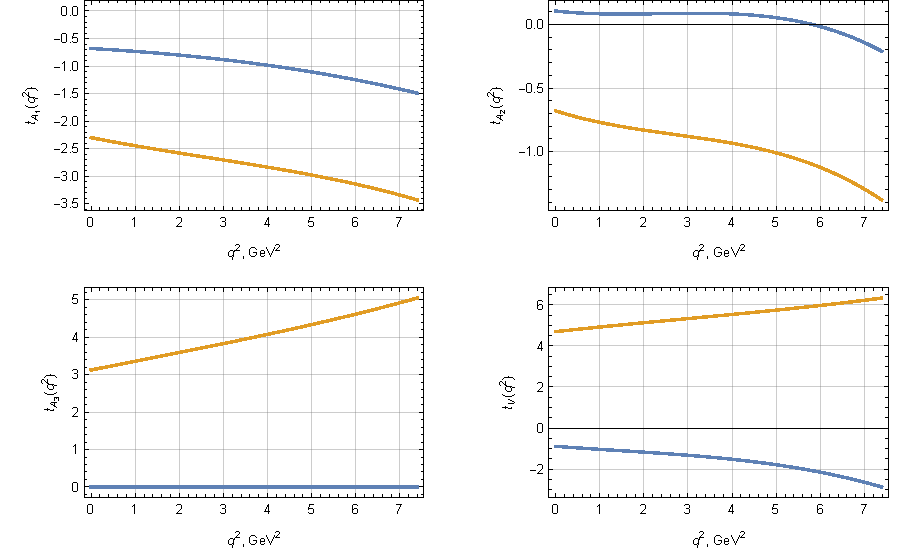
\includegraphics[width=0.7\textwidth]{figs/ff_chi_c2}
\end{center}
\end{frame}

\begin{frame}
  \frametitle{$B_c \to \chi_{c2} \pi$}
  \begin{columns}
    \begin{column}{0.5\textwidth}
      \centering{[Ebert]:}
      % Bc -> chi_c2 + P with [Ebert]
      \begin{tabular}{lcr}
          Paper &:& $\Br  = 0.038\%$ \\
          this      &:& $\Br  = 0.041\%$ \\
		  ratio   &:& $1.078$ \\
      \end{tabular}

    \end{column}
    \begin{column}{0.5\textwidth}
      \centering{[Wang]:}
      % Bc -> chi_c2 + P with [Wang]
      \begin{tabular}{lcr}
          Paper &:& $\Br  = 0.021\pm 0.005\%$ \\
          this      &:& $\Br  = 0.07\%$ \\
		  ratio   &:& $3.331\pm 0.793$ \\
      \end{tabular}

    \end{column}
  \end{columns}
\end{frame}


\begin{frame}[t]
  \frametitle{$B_c \to \chi_{c2} e \nu$}
  \begin{columns}
    \begin{column}{0.5\textwidth}
      \centering{[Ebert]}
      % Bc -> chi_c2 + enu with [Ebert]
      \begin{tabular}{lcr}
          Paper &:& $\Br  = 0.16\%$ \\
          this      &:& $\Br  = 0.16\%$ \\        
      \end{tabular}

      \VSpace 
      \visible<2->{      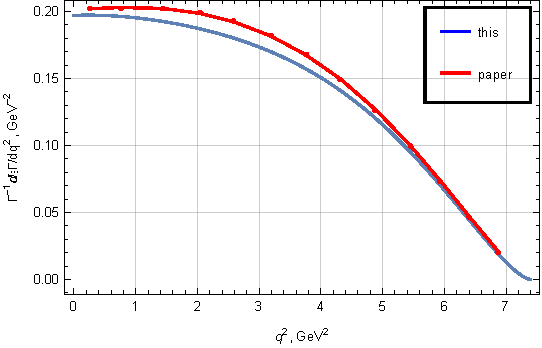
\includegraphics[width=0.9\textwidth, height = 0.55\textheight]{chi_c2_enu_q2_Ebert}}
    \end{column}
    \begin{column}{0.5\textwidth}
      \only<3->{
        \centering{[Wang]}
      % Bc -> chi_c2 + enu with [Wang]
      \begin{tabular}{lcr}
          Paper &:& $\Br  = 0.1\pm 0.03\%$ \\
          this      &:& $\Br  = 0.1\pm 0.03\%$ \\        
      \end{tabular}

      }
      \VSpace 
      \only<3,4>{\visible<4>{      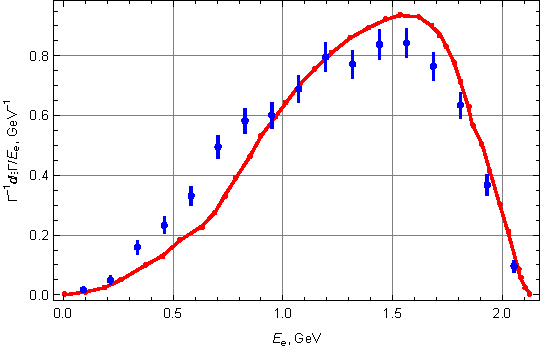
\includegraphics[width=0.9\textwidth, height = 0.55\textheight]{chi_c2_enu_e2_Wang}}}
      \only<5>{      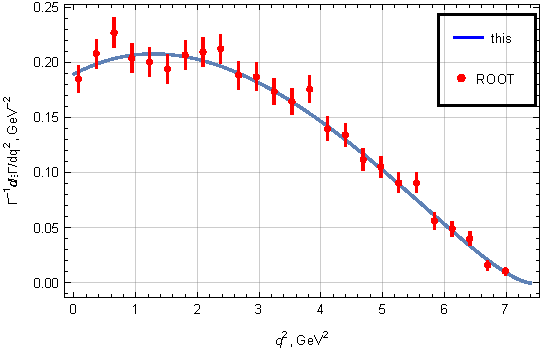
\includegraphics[width=0.9\textwidth, height = 0.55\textheight]{chi_c2_enu_q2_Wang}}
    \end{column}
  \end{columns}
\end{frame}


\begin{frame}
  \frametitle{$B_c \to \chi_{c2} \rho$}
  $$
  \Br\left[B_c \to \chi_{c2} \rho\right] =
  6\pi^2 f_\rho^2 \left.
    \frac{d\Br\left(B_c\to\chi_{c2}+e\nu\right)}{dq^2}
  \right|_{q^2=m_\rho^2}
  $$
  \begin{columns}
    \begin{column}{0.5\textwidth}
      \centering{Ebert}
      \vspace{3mm}
      \centering{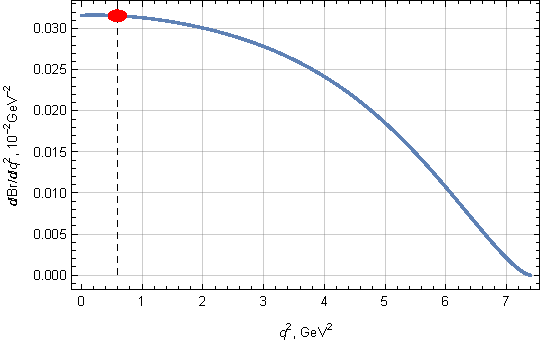
\includegraphics[width=0.9\textwidth]{chi_c2_enu_rho_Ebert}}
      % Bc -> chi_c2 + V with [Ebert]
      \begin{tabular}{lcr}
          Paper &:& $\Br  = 0.11\%$ \\
          this      &:& $\Br  = 0.105\%$ \\
		  ratio   &:& $0.955$ \\
      \end{tabular}

    \end{column}
  \begin{column}{0.5\textwidth}
      \centering{Wang}\\
      \vspace{3mm}
      \centering{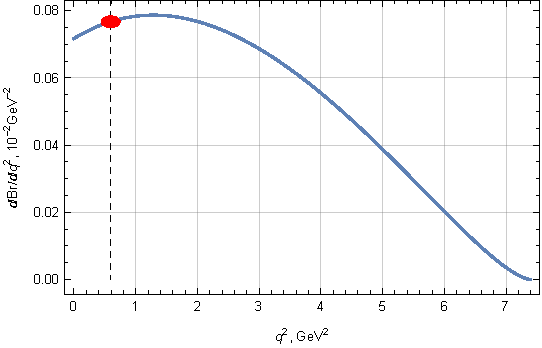
\includegraphics[width=0.9\textwidth]{chi_c2_enu_rho_Wang}}
      % Bc -> chi_c2 + V with [Wang]
      \begin{tabular}{lcr}
          Paper &:& $\Br  = 0.056\pm 0.011\%$ \\
          this      &:& $\Br  = 0.154\%$ \\
		  ratio   &:& $2.754\pm 0.541$ \\
      \end{tabular}

    \end{column}
\end{columns}
\end{frame}


\section{$B_c\to \chi_{cJ}+n\pi$}
\begin{frame}
  \frametitle{$B_c\to \chi_{cJ}+n\pi$}
  $$
  \frac{d\Gamma\left(B_c \to \chi_{cJ} + n\pi\right)}{dq^2} = \frac{d\Gamma\left(B_c \to \chi_{cJ} + n\pi\right)}{dq^2} \frac{\rho_T^{(n\pi)}(q^2)}{\rho_T^{(e\nu)}}
  $$
  Brangings (in $10^{-5}$):
  {\small
    $$
\begin{array}{c|ccc|ccc|ccc}
 \text{} & \chi _{\text{c0}} &  &  & \chi _{\text{c1}} &  &  & \chi _{\text{c2}} &  &  \\
 \text{} & \text{2$\pi $} & \text{3$\pi $} & \text{5$\pi $} & \text{2$\pi $} & \text{3$\pi $} & \text{5$\pi $} & \text{2$\pi $} & \text{3$\pi $} & \text{5$\pi $} \\
\hline
 \text{[Ebert]} & 49.4 & 14.7 & 95.8 & 30.8 & 19.5 & 60. & 3.2 & 4.1 & 5.8 \\
 \text{[Wang]} & 79.8 & 28.2 & 105.4 & 49.4 & 32. & 68. & 4.7 & 5.3 & 6. \\
\end{array}$$

    }
  $q^2$ distributions are approximately the same for all $\chi_{cJ}$
  \centering{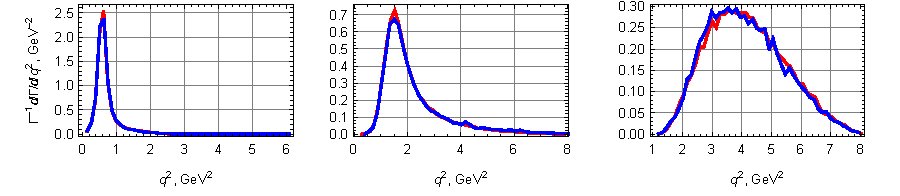
\includegraphics[width=0.9\textwidth]{chi_c0_nPi_q2}}
\end{frame}

\section{EvtGen}
\begin{frame}[fragile]
  \frametitle{EvtGen}
  All described dacays modes are added to BC\_VHAD model
  \begin{itemize}
  \item   Typical decay file:
    \begin{block}{}
\begin{verbatim}
Decay B_c+
  1.000 chi_c0 pi+ pi+ pi+ pi- pi- BC_VHAD 1;
Enddecay
\end{verbatim}
    \end{block}
\item All usual for model out states: $e\nu$, $2\pi$, $3\pi$, $5\pi$, \dots 
\item Particles' order is determined automatically 
\end{itemize}


\end{frame}


\section{Results and Conclusion}
\begin{frame}
  \frametitle{Results' Summary}
  Original branchng fractions:
  {\tiny$$
\begin{array}{r|rr|rr|rr}
  &\multicolumn{2}{c}{\chi_{c0}} & \multicolumn{2}{c}{\chi_{c1}} & \multicolumn{2}{c}{\chi_{c2}} \\
   & \text{[Ebert]} & \text{[Wang]} & \text{[Ebert]} & \text{[Wang]} & \text{[Ebert]} & \text{[Wang]} \\
\hline
 e\nu & 0.087 & 0.13\pm 0.03 & 0.082 & 0.11\pm 0.03 & 0.16 & 0.1\pm 0.03 \\
 \pi & 0.021 & 0.031\pm 0.004 & 0.02 & 0.0021\pm 0.0002 & 0.038 & 0.021\pm 0.005 \\
 \rho & 0.058 & 0.076\pm 0.009 & 0.015 & 0.023\pm 0.002 & 0.11 & 0.056\pm 0.011 \\
\end{array}
$$}
  
  Predicitons for branching fractions of the considered decays
  {\tiny$$
\begin{array}{r|rr|rr|rr}
  &\multicolumn{2}{c}{\chi_{c0}} & \multicolumn{2}{c}{\chi_{c1}} & \multicolumn{2}{c}{\chi_{c2}} \\
   & \text{[Ebert]} & \text{[Wang]} & \text{[Ebert]} & \text{[Wang]} & \text{[Ebert]} & \text{[Wang]} \\
\hline
 e\nu & 0.0889 & 0.138 & 0.0822 & 0.115 & 0.16 & 0.0971 \\
 \pi & 0.0217 & 0.0349 & 0.000644 & 0.00281 & 0.041 & 0.0238 \\
 \rho & 0.0547 & 0.0901 & 0.0127 & 0.0269 & 0.105 & 0.0656 \\
 2\pi & 0.0568 & 0.0935 & 0.0154 & 0.0311 & 0.109 & 0.0684 \\
 3\pi & 0.0213 & 0.0345 & 0.0156 & 0.0249 & 0.041 & 0.0262 \\
 5\pi & 0.0000379 & 0.0000564 & 0.0000486 & 0.0000634 & 0.0000671 & 0.0000391 \\
\end{array}
$$}

  Ratios (this/paper)
  {\tiny$$
\begin{array}{r|rr|rr|rr}
  &\multicolumn{2}{c}{\chi_{c0}} & \multicolumn{2}{c}{\chi_{c1}} & \multicolumn{2}{c}{\chi_{c2}} \\
   & \text{[Ebert]} & \text{[Wang]} & \text{[Ebert]} & \text{[Wang]} & \text{[Ebert]} & \text{[Wang]} \\
\hline
 e\nu & 1.33 & 1.37\pm 0.317 & 1.3 & 1.35\pm 0.369 & 1.3 & 3.79\pm 1.14 \\
 \pi & 1.02 & 1.13\pm 0.145 & 0.031 & 1.31\pm 0.125 & 1.05 & 3.33\pm 0.793 \\
 \rho & 0.726 & 0.917\pm 0.109 & 0.819 & 1.08\pm 0.0942 & 0.738 & 2.75\pm 0.541 \\
\end{array}
$$}
  
\end{frame}

\begin{frame}
  \frametitle{Conclusion}
  \begin{itemize}
  \item Considering $B_c \to \chi_{cJ}+\R$ decays
  \item Factorization model, spectral function approach
  \item Form-factor sets from
    \begin{itemize}
    \item Ebert
    \item Wang
    \end{itemize}
  \item Resonable agreement with papers' results, with some exceptions
    \begin{itemize}
    \item [Ebert]: $B_c\to\chi_{c1}\pi$
    \item [Ebert]: $B_c\to \chi_{cJ}\rho$ vs $B_c\to\chi_{cJ}e\nu$
    \end{itemize}
  \item New results for $R=2\pi, 3\pi, 5\pi$
  \item New decays added to EvtGen model (BC\_VHAD)
  \end{itemize}
\end{frame}


\end{document}
